\documentclass[14pt,fleqn]{extarticle}
\RequirePackage{prepwell-eng}

\previewoff 

\begin{document} 
\begin{snippet}
    
    \incorrect
    
    The area $(A)$ of the region enclosed by the lines $x = y, x + y =2$ and the \xaxis is given by 
    \[ \qquad A = \int_0^1 \left(-x+2 \right)\cdot dx + \int_1^2 x\cdot dx \]
    
    \reason
    
    The required area $(A)$ is as shown in the figure below 
    
    \begin{center}
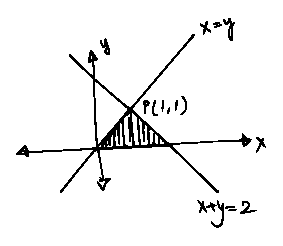
\includegraphics[scale=1.4]{figure.eps}
\end{center}

    The two lines intersect at $P = (1,1)$. Hence, the required area is 
    \[ \qquad A = \int_0^1 x\cdot dx + \int_1^2 \left(-x+2 \right)\cdot dx \]
    
\end{snippet} 
\end{document} 